\chapter{Life-Cycle Energy and Carbon Footprint Modeling with Data Center Building Energy Models}
\label{chp:intro}

\section{Introduction}
    In this chapter, the aim is to quantify the end to end life cycle costs of data centers by extending the operational models developed in the previous chapters. Those operational models have provided an indication of system level energy for a network of data centers and their marginal carbon dioxide footprints. Although, the presented models are a good proxy for the environmental costs of data center operations, they don't account for the energy and carbon footprint embodied in all the materials that the data centers are composed of.

    To assess the end to end environmental impact of data centers, this chapter describes a three-step hybrid life-cycle analysis inclusive of the embodied inventories of the physical data center infrastructure. As the first step, the building energy and marginal costs of energy generation models are reviewed. These two models together provide an indication of the respective costs during the operational phase of a data center's life. Then as the second step, a life cycle modeling framework using an economic input-output (EIO) analysis model extended to environmental costs is introduced. The inputs to the EIO are constructed in this chapter based on literature reviews and the researcher's industrial experience. The final step provides a global view of the end to end assessment by presenting the energy and carbon footprint of each of the data center-language pair analyzed in the previous chapters. With the global view, the global environmental costs of a discrete service can be assessed.

    \subsection{Motivations for an end to end life cycle cost model}
        In terms of scale, US data centers consumed 700 billion kWh in 2016. That was 1.8\% of the total electricity produced in the country according to a United States Department of Energy (DOE) report \cite{Shehabi16}. To drive further intuition of their scale, a typical 100-MW data center at peak load consumes the same amount of energy in an hour as 100 homes do in a month. Given a data centers power demands, it is not surprising that operational energy use has a high sensitivity towards their total cost of ownership (TCO); making it a key metric in TCO based design decisions. While optimization for use phase energy may significantly reduce the carbon footprint of a data center (given the source energy mix does not change), it does not account for other phases in the data center's end to end life cycle. Inventories from embodied life cycle phases such materialization, transit, maintenance, and end of life are left out of the operational phase energy models that have become prevalent indicator of data center sustainability. 

        There are two predominant paradigms for evaluating the embodied environmental inventories for any product that has been altered by technology (techno-sphere). The first method is process based. The complexity of a process-based model is greatly influenced by the boundary conditions of the study. If the boundary is demarcated between the biosphere and the techno-sphere, then the number of distinct life cycle processes to quantify explodes by 500 times for a simple pen \cite{shah11}. The alternate method is based on Leontief's macro-economic proxies that exploits economic correlations between industrial sectors. In macro-economic models, a matrix with rows and columns equal to the number of sectors in the economy is populated with the cost relationship between the row-sector and the corresponding column-sector. Industrial-sector macro-economic proxies reduce the problem space significantly as only one cost vector is required as input to analyze an entire economy. This research combines the two paradigms and presents a hybrid life-cycle assessment model of data centers that can be used to support data center design decisions. 

        The structure of the paper is as follows. First, some technical background about data centers is provided along with a synthesis of similar works. Then in the methodology section a dynamic model to quantify the operational and embodied costs of data center infrastructure is described. The results from the methods as then presented in the results section. This article concludes by summarizing its findings and suggesting the future direction in this area of research. 

\section{Background}
    \subsection{Technical Overview of Data Centers}
        Modern internet data centers are district scale systems, spanning campuses that are hundreds of acres. They may contain several hundred thousand pieces of information technology (IT) equipment. IT equipment consists of physical servers, network hardware nodes, and digital storage media. Theses pieces of IT equipment sit alongside the data center's district scale cooling and electrical distribution plants housed in warehouse-scale built environments. The environmental footprint of a data center spans the full breadth of these physical pieces of infrastructure. 

        At their scale data centers receive power through medium voltage connections with the local utility's grid. The alternating-current voltage may then be stepped down in several steps, but ultimately, it is rectified to be used by the sensitive electronic components in the information technology hardware. Each step-down is a point of power inefficiency, with the alternating-current to direct-current conversion being the biggest point of power loss. Furthermore, anywhere that the step down or conversion occurs inside the building, the electrical inefficiencies are manifested as heat.  

        The heat from the electrical inefficiencies, along with the heat emitted by the IT equipment transistor state transitions and their current leakage, must be rejected to the outside of the building space by mechanical means. At a fundamental level, a mechanically driven fluid mover is needed to convey the heat from indoors to outdoors or another reservoir. In single pass cooling systems fans intake outside-air and force them through the IT equipment, capturing any heat and carrying it outside of the buildings. More complex cooling systems may include liquid or gas refrigerant medium thermodynamic cycles between the buildings and reservoirs, with the refrigerant medium capturing heat at either the building room level or at the scale of IT equipment. Precise modeling of such data center building systems with intense therm-power dynamics is now a manageable task in building energy modeling software \cite{kumar20,kumar20b}. 

        The embodied costs of IT equipment and building systems yield additional environmental costs for a data center's life cycle. The rate of innovation for IT equipment and the ever-increasing demands from the software applications creates a capital market where TCO of one generation of IT hardware rapidly increases relative to newer IT hardware solutions. The capital of cost/performance trade-off makes the positive TCO life of IT equipment between two to five years as observed by Shehabi in the DOE report \cite{Shehabi16}. This relatively short lifetime of IT further compounds the embodied costs of data centers. For example, through a 20-year data center building life, four to ten generations of IT transit through the facility. Disparities in lifetimes and dimensional scale differences between buildings and microchips make data center embodied inventory modeling complex. However, recently hybrid life cycle assessment models have shown to be effective in quantifying the embodied costs of data centers \cite{shah11, whitehead15}. 

        Information technology equipment requires some further insights in order to make its impact to data center life cycle analysis more concrete and directed in scope. At the heart of information technology equipment are microprocessor chips. Modern chips are composed of billions of transistors which have been getting smaller in size since their first applications in electronics signal processing in the 1960's. Transistors have been the key enabler for the compaction and power efficiency gains of electronic devices over the years and they've also been shown to have one of the most dominant environmental costs within electronic products \cite{boyd09, alcaraz18}.

        Prior to the mid-2010's, transistors were composed of planar or 2-D architectures. 2-D transistors inherently had limited operational power efficiencies due to higher voltage and current leakage compared to the novel 3-D processors in the market today. Specifically it's the 3-D processes that have allowed significant operational efficiency gains for data centered operators, yet studies assessing the 3-D transistor architecture's impact to data center life cycle costs are lacking. The 2-D to 3-D transition is a recent example of rapid rate of adaption for information technology equipment that make generalized environmental impacts studies for transducer technology obsolete in two to three years \cite{murphy03}. The frequent churn of technology also drives rapid changes in the manufacturing process of the chips. These rapid changes in semiconductor-manufacturing processes necessitates a parametrically scalable framework where transistor chips can be evaluated in isolation from other server components.  

    \subsection{Similar Works}
        In this section similar works that have quantified the environmental foot print of data centers are presented. Data center life cycle assessment works come from industrial operators \cite{shah11},  academia \cite{whitehead15,kline16}, federal agencies \cite{CLEER13}, and industrial consortium's \cite{tgg12}. Two of the reviewed works are conducive to replicate from the ground up \cite{shah11,whitehead15}, while another serves as a guideline \cite{tgg12}, and another provides an online interactive tool to assess the footprint of targeted classes of Cloud services \cite{CLEER13}. 

        From the operators perspective Shah, demonstrates an end to end life cycle assessment of data center systems \cite{shah11}. Shah uses a hybrid model inclusive of process based and economic input/output assessment frameworks to assess a single a data center, while using a static model for use-phase power. Whitehead, extends Shah's hybrid work and demonstrates the life-cycle costs of a real data center, but with an obscure functional unit \cite{whitehead15}.  
        
        The recent focus on product operational energy efficiency motivated Kline’s study of the trade-offs between operational energy and the embodied costs of information technology equipment \cite{kline16}. Although their bases for the embodied costs are process based, their literature does not provide sufficient insight for others to reproduce the work. Similarly, The Green Grid's Data Center Life Cycle costs guidelines outline the end goal of a data center life cycle analysis. It classifies several key attributes that need to be considered, but lacks references to explicit procedures that must be followed to achieve the goals.  Does this update?
        
       The Cloud Energy and Emissions Research (CLEER) Model provides a browser based user interface to compare the environmental costs of on-premise server based services with hypothetical cloud-based systems that would provide an equivalent service \cite{CLEER13}. CLEER's analysis is transparent and inclusive of embodied and operational costs, but it does not dynamically couple the embodied or operational costs into the model. The presented set of past works has inspired the methodology of this research as described in the next section.

\section{Methodology}
    \subsection{Functional Unit}
    
%     \begin{figure}\centering
    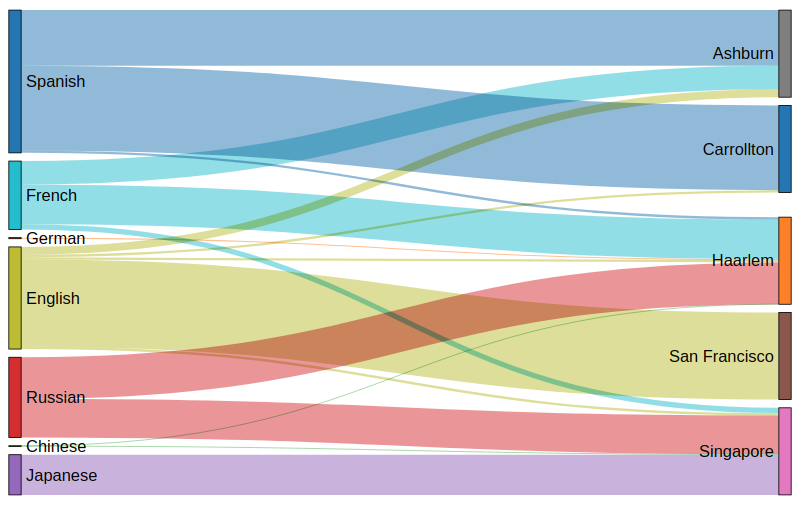
\includegraphics[scale=0.5]{main-chapters/images/lang_dc_sankey.png}
    \caption[Short caption, to appear in the table of contents]{Imported}
    \label{LabelForTheImage}
    \end{figure}
    \begin{figure}\centering
        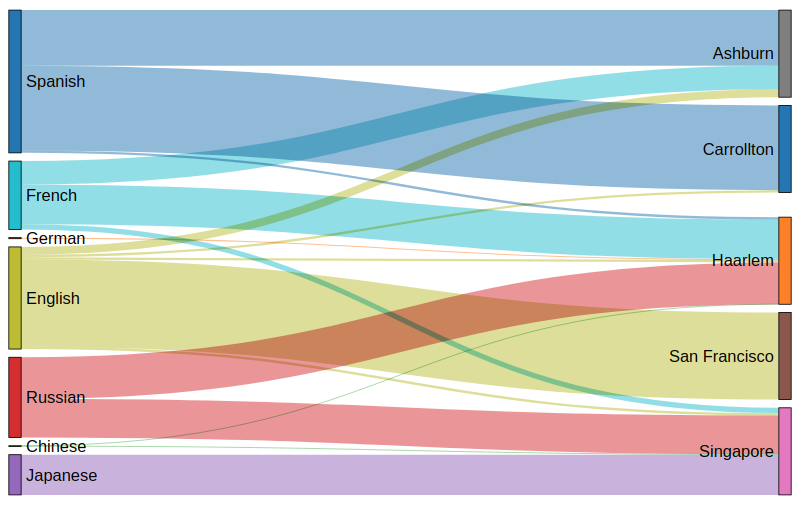
\includegraphics[scale=0.5]{main-chapters/images/lang_dc_sankey.png}
        \caption[Short caption, to appear in the table of contents]{In line.}
        \label{LabelForTheImage}
        \end{figure}

    
    \subsection{System Boundary}
    \subsection{Functional Unit}
    \subsection{System Boundary}
    \subsection{Operational Inventories}
    \subsection{Embodied Inventories}
    l
        \subsubsection{Building Systems}
        \subsubsection{Information Technology Systems}
    
\section{Results}
\section{Discussions}
\section{Conclusion}